% tikzpicture starts at line 1793 of input.tex
\documentclass{standalone}

\usepackage{amsthm, amsmath}

% Prevent the eventual "Too many alphabets" error
\newcommand\hmmax{0}
\newcommand\bmmax{0}

\RequirePackage{notomath}
\RequirePackage{inter}
\RequirePackage[scaled=0.85]{DejaVuSansMono}
\def\bfseries@rm{sb}

\DeclareMathVersion{sansmath}
\SetSymbolFont{operators}{sansmath}{OT1}{NotoSans-TLF}{m}{n}
\SetSymbolFont{letters}{sansmath}{OML}{notosansmi}{m}{it}
\SetMathAlphabet\mathbf{sansmath}{OT1}{NotoSans-TLF}{b}{n}
\SetMathAlphabet\mathsf{sansmath}{OT1}{NotoSans-TLF}{m}{n}
\SetMathAlphabet\mathit{sansmath}{OT1}{NotoSans-TLF}{m}{it}

\DeclareMathVersion{sansmathbold}
\SetSymbolFont{operators}{sansmathbold}{OT1}{NotoSans-TLF}{b}{n}
\SetSymbolFont{letters}{sansmathbold}{OML}{notosansmi}{b}{it}
\SetSymbolFont{symbols}{sansmathbold}{LMS}{ntxsy}{b}{n}
\SetMathAlphabet\mathbf{sansmathbold}{OT1}{NotoSans-TLF}{b}{n}
\SetMathAlphabet\mathsf{sansmathbold}{OT1}{NotoSans-TLF}{b}{n}
\SetMathAlphabet\mathit{sansmathbold}{OT1}{NotoSans-TLF}{b}{it}


% Upright Greek letters uppercase
\DeclareMathSymbol{\Gamma}{\mathord}{operators}{0}
\DeclareMathSymbol{\Delta}{\mathord}{operators}{1}
\DeclareMathSymbol{\Theta}{\mathord}{operators}{2}
\DeclareMathSymbol{\Lambda}{\mathord}{operators}{3}
\DeclareMathSymbol{\Xi}{\mathord}{operators}{4}
\DeclareMathSymbol{\Pi}{\mathord}{operators}{5}
\DeclareMathSymbol{\Sigma}{\mathord}{operators}{6}
\DeclareMathSymbol{\Upsilon}{\mathord}{operators}{7}
\DeclareMathSymbol{\Phi}{\mathord}{operators}{8}
\DeclareMathSymbol{\Psi}{\mathord}{operators}{9}
\DeclareMathSymbol{\Omega}{\mathord}{operators}{10}

% Italic Greek letters lowercase
\DeclareMathSymbol{\alpha}{\mathord}{letters}{11}
\DeclareMathSymbol{\beta}{\mathord}{letters}{12}
\DeclareMathSymbol{\gamma}{\mathord}{letters}{13}
\DeclareMathSymbol{\delta}{\mathord}{letters}{14}
\DeclareMathSymbol{\epsilon}{\mathord}{letters}{15}
\DeclareMathSymbol{\zeta}{\mathord}{letters}{16}
\DeclareMathSymbol{\eta}{\mathord}{letters}{17}
\DeclareMathSymbol{\theta}{\mathord}{letters}{18}
\DeclareMathSymbol{\iota}{\mathord}{letters}{19}
\DeclareMathSymbol{\kappa}{\mathord}{letters}{20}
\DeclareMathSymbol{\lambda}{\mathord}{letters}{21}
\DeclareMathSymbol{\mu}{\mathord}{letters}{22}
\DeclareMathSymbol{\nu}{\mathord}{letters}{23}
\DeclareMathSymbol{\xi}{\mathord}{letters}{24}
\DeclareMathSymbol{\pi}{\mathord}{letters}{25}
\DeclareMathSymbol{\rho}{\mathord}{letters}{26}
\DeclareMathSymbol{\sigma}{\mathord}{letters}{27}
\DeclareMathSymbol{\tau}{\mathord}{letters}{28}
\DeclareMathSymbol{\upsilon}{\mathord}{letters}{29}
\DeclareMathSymbol{\phi}{\mathord}{letters}{30}
\DeclareMathSymbol{\chi}{\mathord}{letters}{31}
\DeclareMathSymbol{\psi}{\mathord}{letters}{32}
\DeclareMathSymbol{\omega}{\mathord}{letters}{33}
\DeclareMathSymbol{\varepsilon}{\mathord}{letters}{34}
\DeclareMathSymbol{\vartheta}{\mathord}{letters}{35}
\DeclareMathSymbol{\varpi}{\mathord}{letters}{36}
\DeclareMathSymbol{\varrho}{\mathord}{letters}{37}
\DeclareMathSymbol{\varsigma}{\mathord}{letters}{38}
\DeclareMathSymbol{\varphi}{\mathord}{letters}{39}

% Change font tracking
\RequirePackage[letterspace=150]{microtype}

% Page breaking
\widowpenalty=10000
\clubpenalty=10000

%%%% Author's definition can start here

\usepackage{tikz}
\usepackage{tkz-graph}
\usepackage{mathdots}
\usepackage{dsfont}
\usetikzlibrary{shapes}

\DeclareMathOperator{\spn}{span}
\DeclareMathOperator{\tr}{tr}
\DeclareMathOperator{\rr}{\mathbb{R}}
\DeclareMathOperator{\cc}{\mathbb{C}}
\DeclareMathOperator{\arity}{arity}
\DeclareMathOperator{\vk}{\mathbf{K}}
\DeclareMathOperator{\vl}{\mathbf{L}}
\DeclareMathOperator{\vg}{\mathbf{G}}
\DeclareMathOperator{\vx}{\mathbf{x}}
\DeclareMathOperator{\vy}{\mathbf{y}}
\DeclareMathOperator{\vz}{\mathbf{z}}
\DeclareMathOperator{\va}{\mathbf{a}}
\DeclareMathOperator{\vb}{\mathbf{b}}
\DeclareMathOperator{\vq}{\mathbf{Q}}
\DeclareMathOperator{\vr}{\mathbf{R}}
\DeclareMathOperator{\vrr}{\mathbf{r}}
\DeclareMathOperator{\vc}{\mathbf{C}}
\DeclareMathOperator{\vcc}{\mathbf{c}}
\DeclareMathOperator{\vj}{\mathbf{J}}
\DeclareMathOperator{\vjj}{\mathbf{j}}
\DeclareMathOperator{\ic}{\mathcal{I}}
\DeclareMathOperator{\fc}{\mathcal{F}}
\DeclareMathOperator{\gc}{\mathcal{G}}
\DeclareMathOperator{\gk}{\mathfrak{G}_{\mathcal{F}}}
\DeclareMathOperator{\qk}{\mathfrak{Q}_{\mathcal{F}}}
\DeclareMathOperator{\stab}{Stab}
\newcommand{\tcwd}[1]{\left\langle #1 \right\rangle_{+, \circ, \otimes ,\top}}
\newcommand{\tcwdn}[1]{\left\langle #1 \right\rangle_{\circ, \otimes ,\top}}
\DeclareMathOperator{\holant}{Holant}
\DeclareMathOperator{\plholant}{Pl-Holant}
\DeclareMathOperator{\csp}{\#CSP}
\DeclareMathOperator{\qut}{Qut}
\DeclareMathOperator{\aut}{Aut}
\DeclareMathOperator{\eq}{\mathcal{EQ}}
\DeclareMathOperator{\geneq}{\mathcal{GEQ}}

\renewcommand*{\VertexSmallMinSize}{6pt}
% draw edges with diamonds in tikz
\newcommand{\DEdge}[2]{
    \draw[thick] (#1) -- (#2) node[draw, fill=white, kite, kite vertex angles = 120, minimum size = 4pt, inner sep = 1pt, pos=0.3, sloped] {};
}


\begin{document}
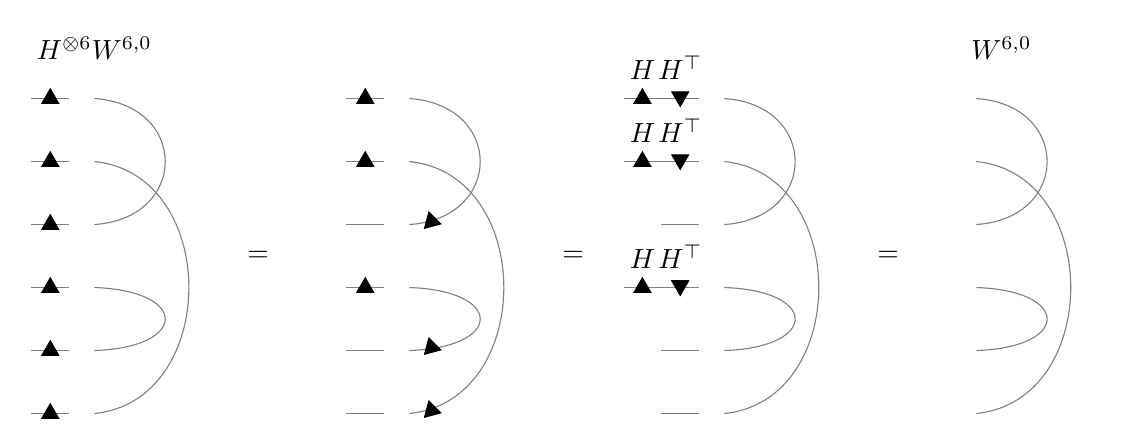
\begin{tikzpicture}[scale=0.8]
    \tikzset{VertexStyle/.style = {shape=circle, fill=black, minimum size=5pt, inner sep=1pt, draw}}
    \GraphInit[vstyle=Classic]
    \SetUpEdge[style=-]
    \SetVertexMath

    % x coordinate of dangling ends
    \def\dx{2}

    \node at (\dx+2.6, 2.5) {$=$};
    \node at (3.5*\dx+2.6, 2.5) {$=$};
    \node at (6*\dx+2.6, 2.5) {$=$};

    \node at (\dx, 5.8) {$H^{\otimes 6} W^{6,0}$};
    \node at (8*\dx+0.4, 5.8) {$W^{6,0}$};

    \foreach \iy in {0,1,...,5} {
        \draw[thin, color=gray] (\dx-1,\iy) -- (\dx-0.4,\iy);
        \node[draw, fill=black, regular polygon, regular polygon sides=3, minimum size = 7pt, inner sep = 1pt] at (\dx-0.7,\iy) {};
    }

    \foreach \ix in {1,3.5,6,8} {
        \draw[thin, color=gray] (\dx*\ix,3) .. controls (\dx*\ix+1.5,3.1) and (\dx*\ix+1.5,4.9) .. (\dx*\ix,5);
        \draw[thin, color=gray] (\dx*\ix,0) .. controls (\dx*\ix+2,0.2) and (\dx*\ix+2,3.8) .. (\dx*\ix,4);
        \draw[thin, color=gray] (\dx*\ix,1) .. controls (\dx*\ix+1.5,1.05) and (\dx*\ix+1.5,1.95) .. (\dx*\ix,2);
    }

    \foreach \iy in {2,4,5} {
        \draw[thin, color=gray] (3.5*\dx-1,\iy) -- (3.5*\dx-0.4,\iy);
        \node[draw, fill=black, regular polygon, regular polygon sides=3, minimum size = 7pt, inner sep = 1pt] at (3.5*\dx-0.7,\iy) {};
    }
    \foreach \iy in {0,1,3} {
        \draw[thin, color=gray] (3.5*\dx-1,\iy) -- (3.5*\dx-0.4,\iy);
        \node[draw, fill=black, rotate=15, regular polygon, regular polygon sides=3, minimum size = 7pt, inner sep = 1pt] at (3.5*\dx+0.35,\iy+0.05) {};
    }

    \foreach \iy in {0,1,3} {
        \draw[thin, color=gray] (6*\dx-1,\iy) -- (6*\dx-0.4,\iy);
    }
    \foreach \iy in {2,4,5} {
        \draw[thin, color=gray] (6*\dx-1.6,\iy) -- (6*\dx-0.4,\iy);
        \node[draw, fill=black, regular polygon, regular polygon sides=3, minimum size = 7pt, inner sep = 1pt, label={[label distance=-0.2mm]$H$}] at (6*\dx-1.3,\iy) {};
        \node[draw, fill=black, rotate=180, regular polygon, regular polygon sides=3, minimum size = 7pt, inner sep = 1pt, label={[label distance=0.2mm]below:$H^\top$}] at (6*\dx-0.7,\iy+0.03) {};
    }
\end{tikzpicture}

    \pagestyle{empty}
    \centering

 

\end{document}
%%% Local Variables:
%%% mode: latex
%%% TeX-master: t
%%% End:
